\documentclass{article}
\usepackage[margin=1in]{geometry}
\usepackage{xcolor}
\usepackage{adjustbox}
\usepackage{verbatim}
\definecolor{shadecolor}{rgb}{.9, .9, .9}
\usepackage{tcolorbox}
\usepackage[colorlinks = true,
            linkcolor = blue,
            urlcolor  = blue,
            citecolor = blue,
            anchorcolor = blue]{hyperref}

\newenvironment{code}%
   {\par\noindent\adjustbox{margin=1ex,bgcolor=shadecolor,margin=0ex \medskipamount}\bgroup\minipage\linewidth\verbatim}%
   {\endverbatim\endminipage\egroup}


%\DeclareUrlCommand{\burl}{\def\UrlFont{\ttfamily\color{blue}}}

\newcommand{\burl}[3][blue]{\href{#1}{\color{#2}{#3}}}%

\title{Conducting experiments on Prolific via Proliferate}
\author{Shawn Cummings, Florian Jaeger, Maryann Tan}

\begin{document}

\maketitle

\tableofcontents

\section{Overview}

This tutorial walks you through how to sandbox your experiment on Proliferate's sandbox, how to upload the (thoroughly tested) experiment to Prolific, and how to collect your data once all assignments have been completed. This tutorial does {\em not} describe how to program your own experiment.

\begin{figure}[htbp]
\begin{center}
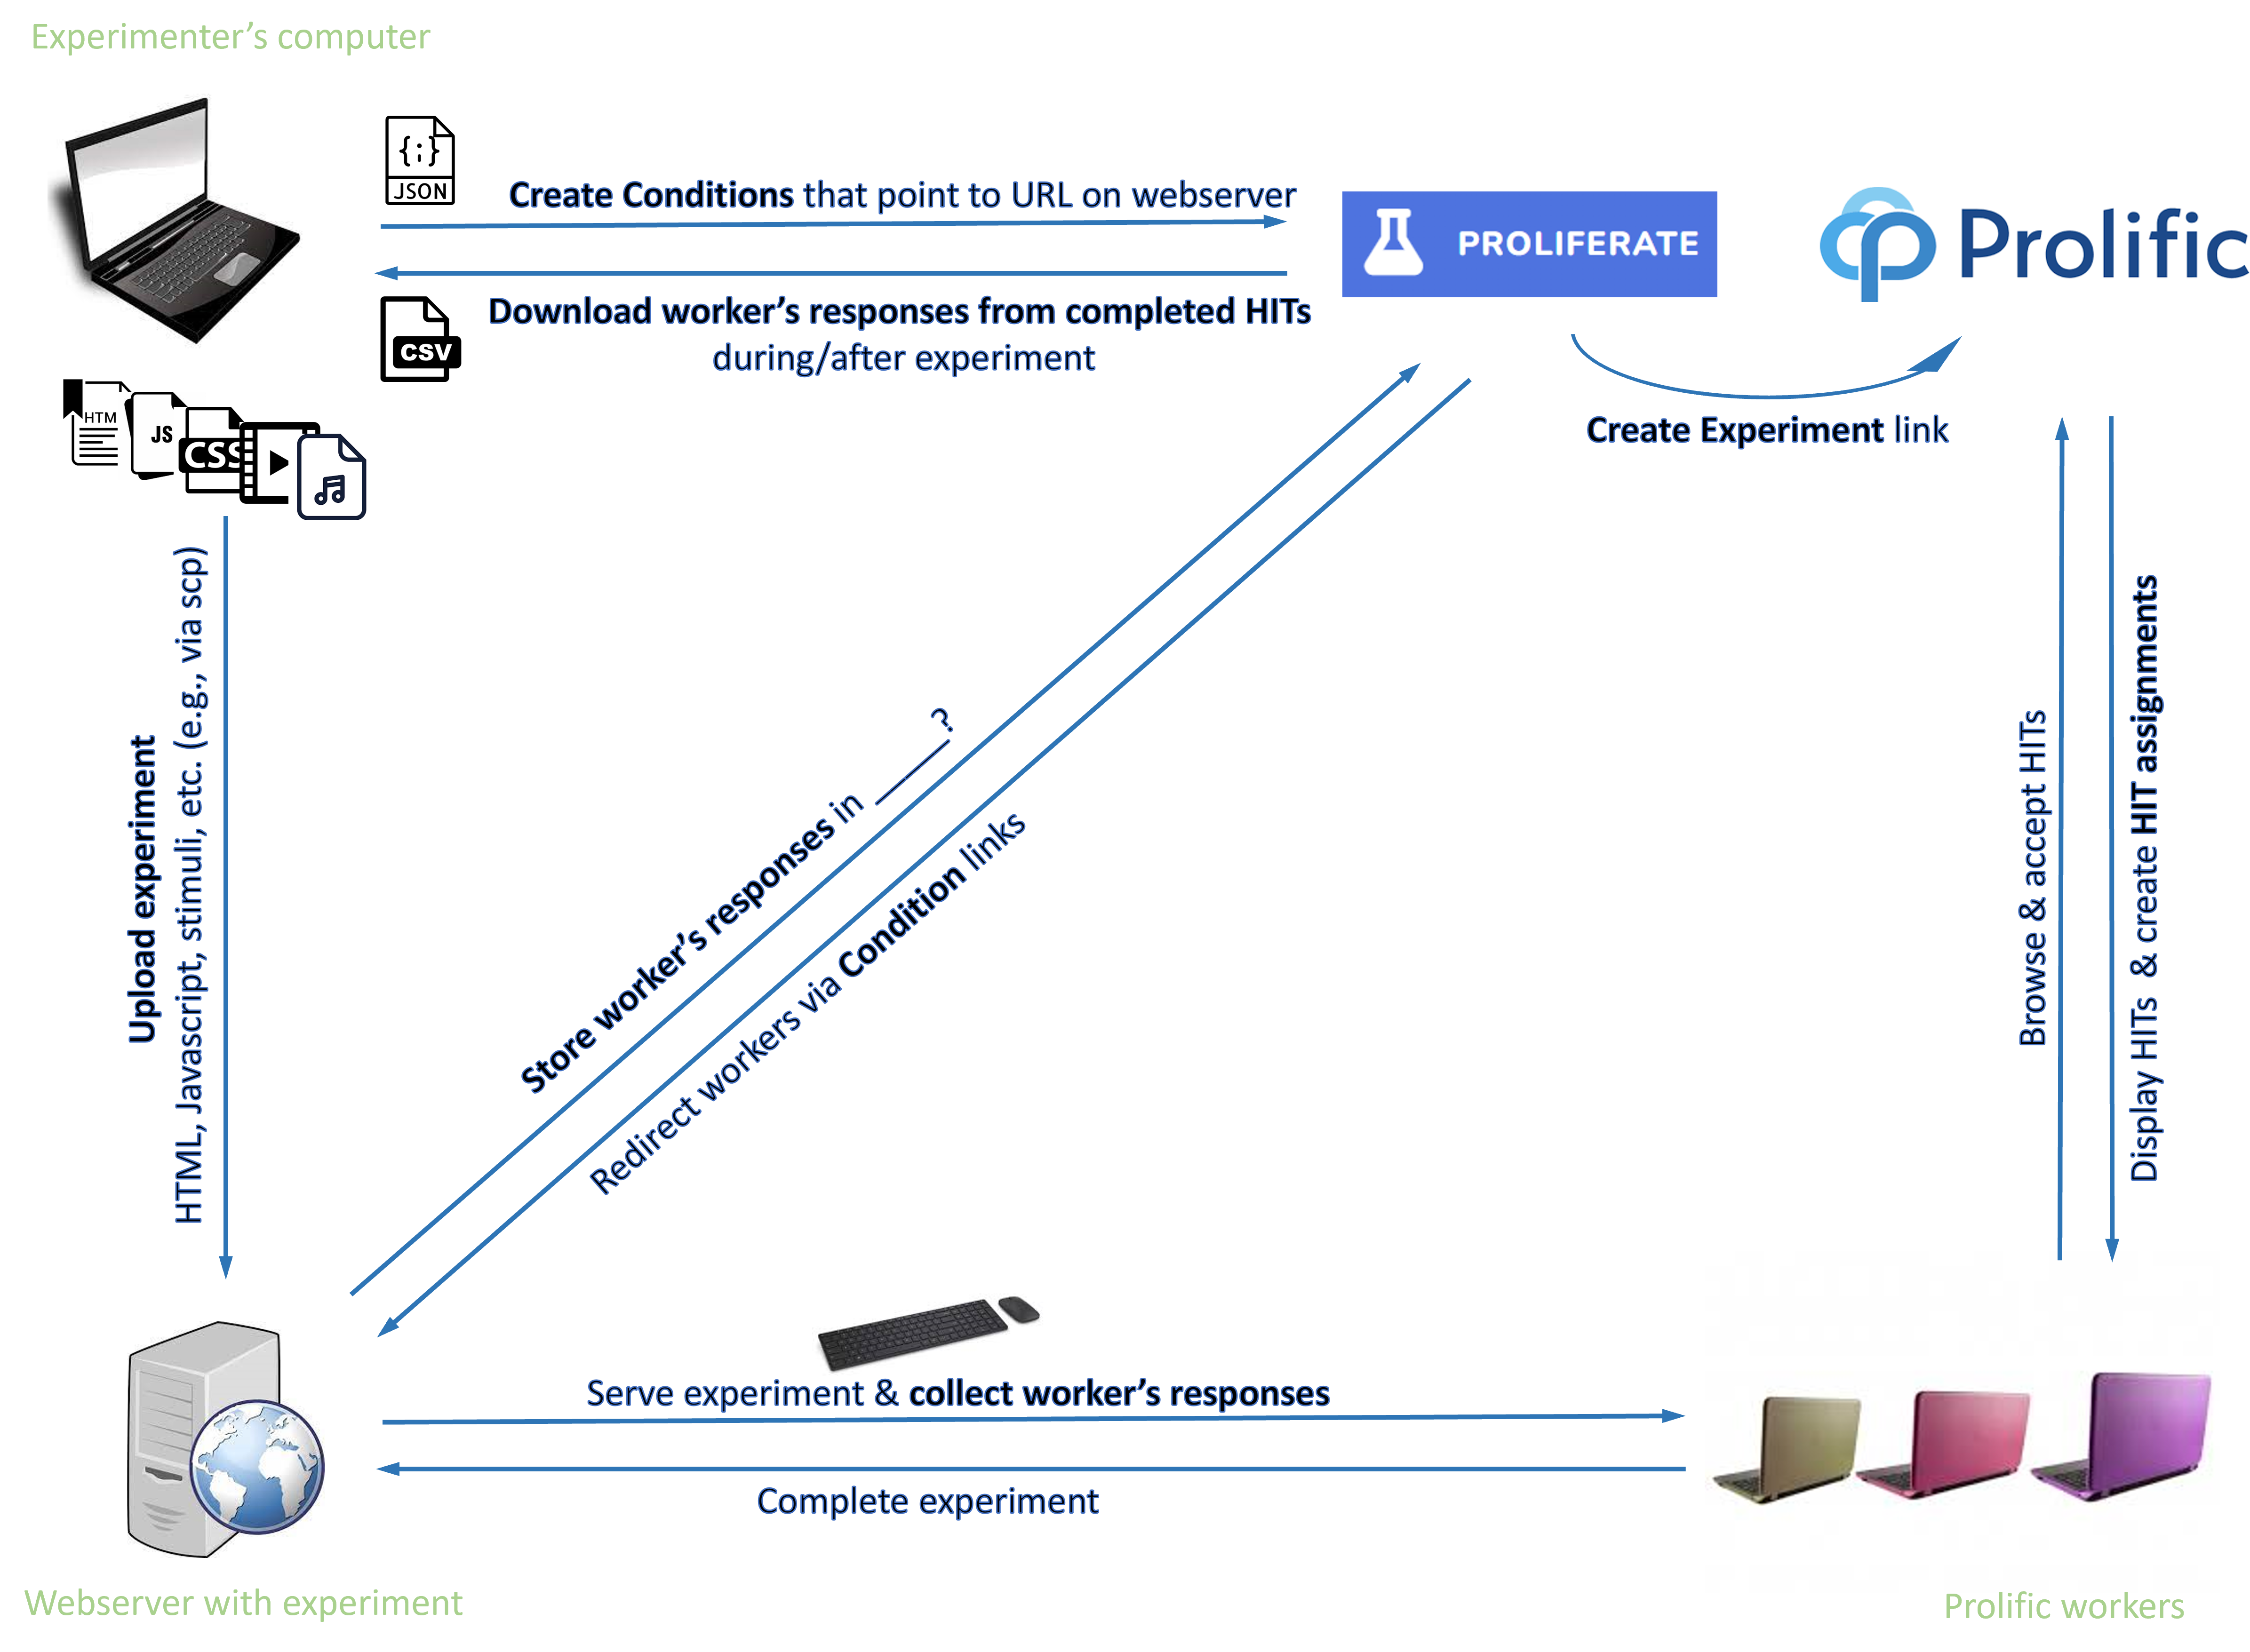
\includegraphics[width=.9\textwidth]{figures/vis_infoflow_prolific.png}
\caption{Overview of how your computer and the web server hosting your experiment interact with each other, Proliferate, and Prolific. MORE DETAILS HERE}\label{fig:overview}
\label{default}
\end{center}
\end{figure}

Figure \ref{fig:overview} provides an overview of the way that your computer and web server will interact with Proliferate and Prolific. The rest of the document describes how this interaction is achieved. 


\section{Prolific and Proliferate}

Prolific (\url{https://prolific.co/}) is an online platform that hosts and distributes experiments to a participant pool. Unlike MTurk, it does not store participant data. Additionally, it does not embed experiments in a frame, but rather simply redirects. 

Proliferate (\url{https://proliferate.alps.science/admin/}) is a tool that facilitates running JavaScript-based experiments on Prolific. It provides a server to store data, and allows (via a .json file, or via 'CONDITIONS' in the GUI) for stratification from a single Prolific link to multiple URLs. For more details and helpful documentation, see /url{https://docs.proliferate.alps.science/en/latest/} 

Before doing further, one should create a free account (or secure access to lab accounts) for both Prolific and Proliferate.

\section{Develop and debug your experiment locally}

After you have completed the HTML (and potentially Javascript or other) programming necessary for your experiment, the first recommended step is to debug the experiment locally on your computer. In many cases, you will not even need to install a local webserver on your computer. If your experiment does not record speech, video, or alike but only {\em presents} audio, video, or other stimuli then you likely will be able to simply open your HTML file on your computer in a browser. This allows you to go through your experiment and debug it. \textbf{Only after you have completed local debugging of your experiment, is it time to test whether your experiment also works on MTurk.}



\end{document}
